\documentclass[pdftex,ptm,14pt,a4paper]{extreport}
\usepackage{float}
\usepackage[utf8]{inputenc}

\usepackage[russian,english]{babel}
    \addto{\captionsenglish}{\renewcommand{\bibname}{Литература}}
    \addto\captionsenglish{\renewcommand{\figurename}{Рис.}}
    \addto\captionsenglish{\renewcommand{\contentsname}{Содержание}}
    \addto\captionsenglish{\renewcommand{\proofname}{Доказательство}}
\usepackage[T2A]{fontenc}

\makeatletter
\renewcommand*{\ps@plain}{%
  \let\@mkboth\@gobbletwo
  \let\@oddhead\@empty
  \def\@oddfoot{%
    \reset@font
    \hfil
    \thepage
    % \hfil % removed for aligning to the right
  }%
  \let\@evenhead\@empty
  \let\@evenfoot\@oddfoot
}

\usepackage{csquotes}

\usepackage[backend=bibtex]{biblatex}
\bibliography{draft}

\makeatother
\pagestyle{plain}
\usepackage{amsthm}
\usepackage{mathtools}
\usepackage{caption}
\usepackage{subcaption}
\usepackage{cmap}
\usepackage{verbatim}
\usepackage[table,xcdraw]{xcolor}

\usepackage{amsfonts}
\usepackage{amsmath}
\usepackage{amssymb}
\usepackage{listings}
\usepackage{graphicx}

%\usepackage{bbm, dsfont}


\makeatletter
\renewcommand{\@chapapp}{Часть}
\makeatother

% Theorem Styles
\newtheorem{theorem}{Теорема}[chapter]
\newtheorem{lemma}[theorem]{Лемма}
\newtheorem{claim}[theorem]{Теорема}
% Definition Styles
\theoremstyle{definition}
\newtheorem{definition}{Определение}[chapter]
\newtheorem{example}{Пример}[chapter]

\newcommand{\HRule}{\rule{\linewidth}{0.5mm}}

%\usepackage{minted}
\graphicspath{ {/home/ssmike/sem/report/} }
%\includegraphics[scale=0.5]{name.png}

%\inputminted{syntax}{code}

% \begin-end{lstlisting}
\catcode`@=11
\def\caseswithdelim#1#2{\left#1\,\vcenter{\normalbaselines\m@th
  \ialign{\strut$##\hfil$&\quad##\hfil\crcr#2\crcr}}\right.}% you might like it without the \strut
\catcode`@=12
%
\def\bcases#1{\caseswithdelim[{#1}}
\def\vcases#1{\caseswithdelim|{#1}}
%

\title{}
\author{М.С. Сурин}
\DeclareMathOperator{\sgn}{sgn}

\begin{document}
\begin{comment}
    \begin{titlepage}
    \newpage

    \begin{center}
    МИНИСТЕРСТВО ОБРАЗОВАНИЯ И НАУКИ РОССИЙСКОЙ ФЕДЕРАЦИИ \\
    \vspace{0.5cm}
    ГОСУДАРСТВЕННОЕ ОБРАЗОВАТЕЛЬНОЕ УЧРЕЖДЕНИЕ \\*
    ВЫСШЕГО ПРОФЕССИОНАЛЬНОГО ОБРАЗОВАНИЯ\\*
    "МОСКОВСКИЙ ФИЗИКО-ТЕХНИЧЕСКИЙ ИНСТИТУТ \\*
    (ГОСУДАРСТВЕННЫЙ УНИВЕРСИТЕТ)" \\*
    \vspace{0.5cm}
    ФАКУЛЬТЕТ ИННОВАЦИЙ И ВЫСОКИХ ТЕХНОЛОГИЙ \\*
    КАФЕДРА АНАЛИЗА ДАННЫХ \\*
    \hrulefill
    \end{center}


    \vspace{8em}

    \begin{center}
    \Large Выпускная квалификационная работа по направлению 01.03.02 <<Прикладные математика и информатика>> \linebreak НА ТЕМУ:
    \end{center}

    \vspace{2.5em}

    \begin{center}
    \textsc{\large{\textbf{TITLE}}}
    \end{center}

    \vspace{6.5em}

    \begin{flushleft}
        Студент \hrulefill Сурин М.С.  \\
    \vspace{1.5em}
        Научный руководитель к.ф-м.н \hrulefill Артемов А.В.\\
    \vspace{1.5em}
    Зам. зав. кафедрой д.ф-м.н, профессор \hrulefill Бунина Е.И.
    \end{flushleft}

    \vspace{\fill}

    \begin{center}
    МОСКВА, 2017
    \end{center}

    \end{titlepage}
\end{comment}

\tableofcontents

\sloppy

\chapter{Введение}
Тестирование распределённых и устойчивых к сбоям баз данных является более сложной задачей чем тестирование монолитных систем

В силу асинхронности сети(\cite{network-reliable}) и возможности аппаратных сбоев разработка распределённых и устойчивых к сбоям
баз данных является более сложной задачей чем разработка монолитных систем. Поэтому, требуется более тщательное тестирование,
проверяющее отказоустойчивость и выполнение декларируемых гарантий в случае сбоев отдельных узлов и каналов связи между ними.
В данной работе используется метод внесения неисправностей(fault injection) для верификации подсистем Yandex.YT.

Yandex.YT является map-reduce системой, которую так или иначе используют практически все сервисы Yandex.
В том числе, многие сервисы реального времени хранят данные в подсистеме YT, которую мы тестируем в данной работе.
В нем хранятся такие данные как показы рекламы, данные клиентов,\dots. Поэтому, нарушение заявляемых гарантий может
привести к поломке или простою критически важных процессов. И последующей потере денег

\chapter{Обзор литературы}
В данной главе сделан обзор существующих методов
верификации гарантий консистентности распределённых систем.

\section{Формальные спецификации}
Метод формальных спецификаций заключается в построении математической модели системы, формализации требований к ней и последующему
доказательству того, что система удовлетворяет поставленным требованиям. Обычной практикой является использование инструментов, позволяющих получить доказательство в полуавтоматическом режиме(\cite{coq}).
Построение формальных спецификаций полезно при доказательстве корректности модели соответствующей
системы, но  в случае, если модель оказывается достаточно громоздкой, возникают вопросы
соответствия этой модели реальной системе, а также проблемы обновления модели при изменении её функциональности.
Данные ограничения, как отмечают авторы в \cite{models-bounds} сильно повышают стоимость поддержки
и делают данный подход оправданным только для критичных систем.
Впрочем, достаточно большие компании, такие как Amazon, всё-таки могут позволить себе использование формальных моделей
(\cite{amazon-formal-proofs}) наряду с другими методами.

\section{Внесение неисправностей}
Метод внесения неисправностей заключается в искусственном создании неисправностей(аппаратных сбоев), направленном на
тестирование отказоустойчивости системы. Применительно к распределённым системам это такие неисправности, как искусственные разрывы сети или
отказы вычислительных узлов. В отличие от построения спецификаций данный метод не позволяет доказать корректность, но является гораздо менее накладным, а так же не оперирует с производными от конечного продукта(формальной моделью), что расширяет область применения.
Netflix использует этот подход(\cite{netflix-simian-army}) для тестирования своих сервисов.
Многие системы с открытым исходным кодом тестировались при помощи фреймворка jepsen(\cite{jepsen-io}, \cite{jepsen-analyses}), который
упрощает внесение неисправностей(искусственные разрывы сети, и т.д.).
Также существуют примеры применения
гибридных методик, такие как lineage-driven fault injection(\cite{molly}) -- когда вместо того, чтобы тестировать
систему методом чёрного ящика, используется знание протокола, и избирательно теряются сообщения между узлами.
\chapter{Постановка задачи}
В данной работе мы верифицируем подсистемы Yandex.YT, а именно “Кипарис” и “Динамические таблицы”.
Существуют следующие типы нарушений консистентности, которые необходимо обнаружить.
\begin{itemize}
    \item Потеря подтверждённых записей.
    \item Чтение устаревшего состояния.
    \item Чтение данных, появившихся в результате неподтверждённых записей.
\end{itemize}

\section{Кипарис}
“Кипарис” -- распределённое хранилище \guillemotleftключ-значение\guillemotright.
Является CP системой в смысле CAP-теоремы и гарантирует линеаризуемость \cite{linearizable}.

\begin{figure}
    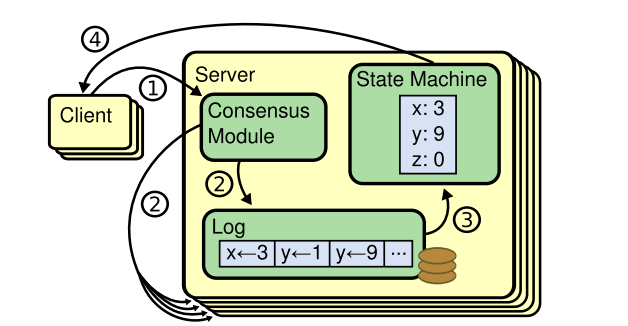
\includegraphics[scale=0.6]{state-machine.png}
\caption{Общая схема системы, построенной по принципу репликации конечного автомата}
\end{figure}

“Кипарис” использует подход репликации конечного автомата\cite{state-replication} и
отказоустойчивость ему придаёт слой репликации называющийся “Hydra”, алгоритм работы которого схож с идеями,
применёнными в Zookeeper \cite{zookeeper} и Raft \cite{raft}.

Опишем в общих чертах алгоритм “Hydra.”
Кластер состоит из $2n+1$ машин.
У каждого узла есть 3 режима работы: лидер, последователь и режим восстановления.

\begin{figure}
    \centering
    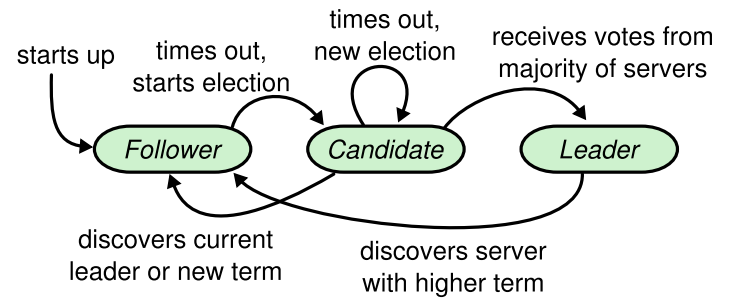
\includegraphics[scale=0.6]{raft-states.png}
    \caption{Переходы между состояниями узлов.}
\end{figure}

Лидер определяется в процессе голосования, которое устроено следующим образом:
\begin{enumerate}
    \item Узлы рассылают всему кластеру длину записанной истории и свой идентификатор,
    \item Узлы выбирают лидера (узел с наименьшим идентификатором среди имеющих наибольшую длину истории)
        и рассылают остальным идентификатор выбранного лидера.
    \item Узел, за которого проголосовали не менее $n+1$ узлов становится лидером.
\end{enumerate}

\begin{figure}
    \centering
    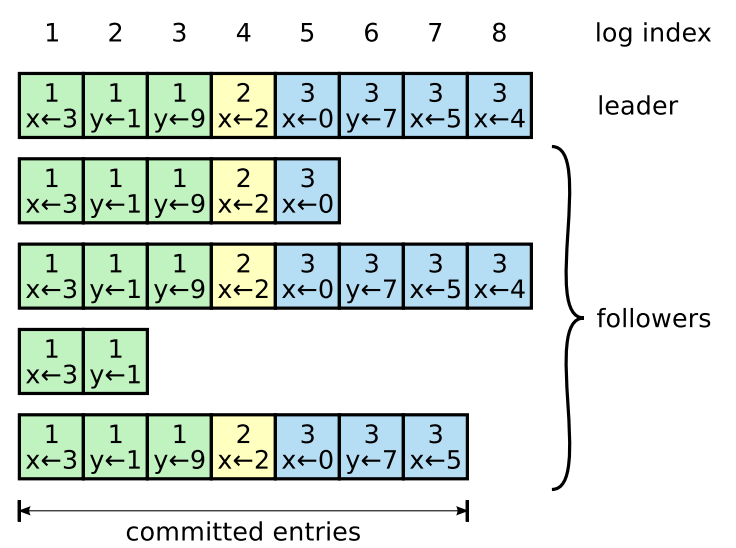
\includegraphics[scale=0.5]{raft-logs.png}
    \caption{Лог операций, хранящийся на каждом узле, состоит из записей, содержащих номер эпохи
             и операцию над состоянием автомата.}
\end{figure}

\begin{figure}
    \centering
    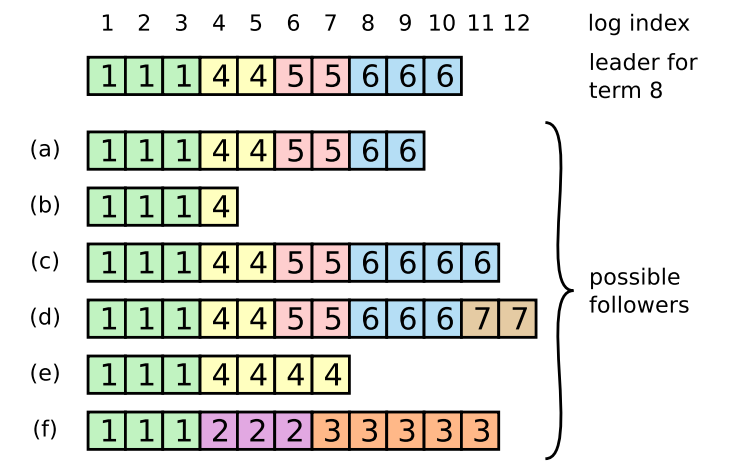
\includegraphics[scale=0.5]{raft-election.png}
    \caption{Выборы лидера. Каждый квадрат обозначает запись в логе. (a-f) -- возможные состояния последователей.}
\end{figure}

Далее каждый узел хранит идентификатор лидера.
Периодически лидер опрашивает последователей, и если не набирается $n$ узлов, для которых верно,
что идентификатор их лидера совпадает с опрашивающим узлом, то начинаются выборы.
Также выборы начинаются, если в течение заранее заданного промежутка времени какой-либо из последователей не был опрошен лидером.

При записи (любом мутирующем запросе) клиент обращается к лидеру, который в свою очередь опрашивает последователей и
реплицирует на них запрос. Лидер отвечает успехом если по крайней мере $n$ последователей подтвердили что их хранимый идентификатор
лидера совпадает с опрашивающим узлом, и они записали изменение на диск.

На запросы чтения лидер отвечает без подтверждения от последователей.
Последователи отвечают на запрос чтения только после того как получено подтверждение от лидера о том, состояние узла не отстаёт от лидера.
Узлы в режиме восстановления на запросы чтения не отвечают. Более того, узлы в режиме восстановления не голосуют при выборах, а только
асинхронно забирают изменения с лидера.

\section{Динамические таблицы}
“Динамические таблицы” -- это также CP-хранилище
\guillemotleftключ-значение\guillemotright,
в свою очередь являющееся Snapshot-сериализуемым\cite{snapshot-serializable}.
В отличие от линеаризуемости, которая даёт гарантии для операций над одним объектом,
Snapshot-сериализуемость даёт гарантии относительно групп объектов и групп операций над ними,
объединённых в транзакции.
Также отметим отличия от сериализуемости и строгой сериализуемости, которые дают гарантии атомарности
транзакций. В случае snapshot-сериализуемости мы гарантируем что все запросы оперируют с состоянием базы
на момент старта транзакции и то что изменения сделанные внутри транзакции не уничтожат
записи сделанные с начала старта из других транзакций.
Чтобы показать что snapshot-сериализуемость отличается от сериализуемости рассмотрим следующий пример истории:
\begin{gather*}
1:start \\
1:read(2) \\
2:start \\
2:read(1) \\
1:write(1) \\
1:commit \\
2:write(2) \\
2:commit \\
\end{gather*}

Здесь операции сделанные внутри транзакции $x$ помечены как $x:,$ $read(x)$ -- операция чтения из регистра $x,$
$write(x)$ -- некоторая запись в $x.$ $start$ и $commit$ -- начало и завершение транзакции соответственно.
Очевидно, что данная история не является сериализуемой, так как тразакция 2 оперирует с значением в регистре 1
до записи сделанной в транзакции 2, а чтение внутри транзакции 1 сделано до записи внутри транзакции 2.
Подобное ослабление гарантий позволяет добиться повышения производительности и применяется в таких базах
данных как Oracle, Postgres\cite{postgres}, Microsoft SQL Server, Google Spanner\cite{spanner}, Cockroach DB.

Опишем в общих чертах схему работы “динамических таблиц”.

Пространство ключей статически шардировано. Для координации используется “Hydra”.
А именно, для хранения информации о шардах и предоставления монотонных timestamp-меток.
В "рабочем" режиме у каждый шард обслуживает некоторый узел.
Через него проходят все операции на соответствующем диапазоне ключей.
Для обеспечения отказоустойчивости, обслуживающий узел реплицирует историю операций
на кворум из некоторых вторичных для этого шарда узлов.

\begin{figure}[h]
    \centering
    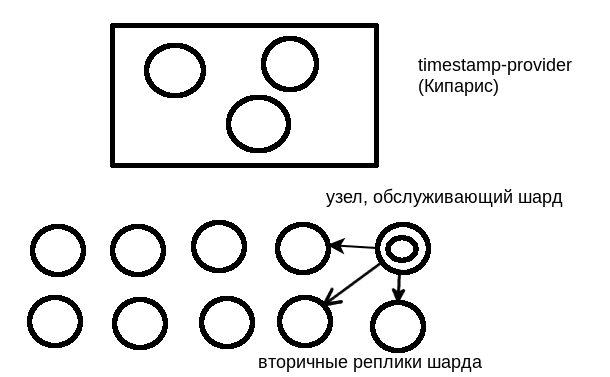
\includegraphics[scale=0.5]{storage.png}
    \caption{Общая схема кластера}
\end{figure}

В данной работе мы тестируем транзакции, которые устроены следующим образом:
В начале транзакции клиент получает timestamp и все чтения в рамках транзакции
производит по нему же. Чтение возвращает наиболее свежую версию данных до полученного
timestamp. При завершении транзакции возможно два принципиально разных случая:
\begin{itemize}
    \item В случае если записи затрагивают 1 шард, этот же шард просто выполняет записи.
    \item В случае если записи затрагивают несколько шардов, используется алгоритм
        двухфазного коммита \cite{tanenbaum2007distributed}.
        А именно,
        \subitem Клиент отправляет запрос всем затронутым шардам, содержащий информацию
            о множестве ключей и timestamp, соответствующий началу транзакции.
        \subitem После получения положительного ответа от всех участников,
            случайный шард назначается координатором и на него же клиент отправляет
            запрос на коммит.
        \subitem Координатор отправляет запрос на подготовку коммита всем участникам.
        \subitem После подтверждения всеми участниками, генерируется timestamp и
            отправляется подтверждение всем участникам.
        \subitem После получения подтверждения от всех участников, отправляется ответ клиенту.
\end{itemize}

\chapter{Предложенный алгоритм}
В данной работе мы пользуемся фреймворком jepsen(\cite{jepsen-io}).
Общая схема процедуры верификации такова:
В несколько потоков делаются серии запросов к базе, развёрнутой на кластере размера 3-5.
Запросы и ответы собираются в единую последовательную историю событий, которая в дальнейшем
 проверяется на соответствие заявленным гарантиям.

\section{jepsen}
Jepsen представляет собой библиотеку для написания тестов и состоит из следующих частей:
\begin{itemize}
    \item \textbf{core} -- основной модуль, управляющий установкой и настройкой тестируемой базы,
        запуском потоков, инициирующих запросы к базе. Запросы, а также моделируемые неисправности
        генерируются при помощи данного на вход  генератора и инициируются данным модулем.
        Также передаёт полученную историю модулю \textbf{checker}, и генерирует отчёт.
    \item \textbf{gen} -- модуль, предназначенный для генерации запросов, неисправностей и т.п..
        Представляет из себя набор элементарных генераторов и операторы для их комбинирования.
    \item \textbf{nemesis} -- модуль для внедрения неисправностей, предназначен для запуска
        отдельного рабочего потока, который создаёт искусственные разрывы сети между узлами,
        имитирует сбои отдельных узлов, манипулирует со временем на узлах и т.п..
    \item \textbf{model} -- Предоставляет модель состояния базы, предназначен для проверки правильности результатов запросов.
    \item \textbf{checker} -- Модуль для интеграции пользовательских анализаторов истории с jepsen.
\end{itemize}

\section{Верификация истории}
\subsection{Кипарис}
\label{cypress-verify}
Для верификации линеаризуемости используется классический алгоритм J. Wing, C.Gong \cite{wing-testing}
с дополнениями G. Lowe \cite{lowe-testing} и A. Horn \cite{horn-faster}.
Приведём краткую схему работы алгоритма.
\begin{definition}[Модель]
    Для множеств $\Xi, \Delta,$, множества операций $\chi \subset ((\{\perp \} \cup \Xi) \times \Delta)^\Xi$
    будем называть $\langle \Xi, \Delta, \chi \rangle$ моделью.
\end{definition}

Неформально -- модель это набор состояний разделяемого объекта($\Xi$) и поддерживаемые операции над ним($\chi$).
$\perp$ означает что операция над данным состоянием объекта не поддерживается. $\Delta$ здесь некоторое множество
выходных значений соответствующих операциям.

\begin{definition}[История]
    Для модели $\langle \Xi, \Delta, \chi \rangle$ будем называть историей последовательность событий вида
    \begin{itemize}
        \item \textit{call.process.op}, где process --  идентификатор процесса,
             $\textit{op}: \in \chi$  -- производимая операция над состоянием разделяемого объекта.
        \item \textit{ret.process.response} process -- идентификатор процесса,
            $\textit{response} \in  \{\textbf{fail},\textbf{ok},\textbf{info}\} \times \Delta$
            %\langle \textit{status}, \textit{value} \rangle,
            %$\textit{response} = \langle \textit{status}, \textit{value} \rangle,
            %\textit{value} \in \Delta,
            %\textit{status} \in \{\textbf{fail},\textbf{ok},\textbf{info}\}$

            Здесь и далее
        \subitem \textit{fail} -- детерминировано отвергнутая операция,
        \subitem \textit{ok} -- успешная операция.
        \subitem \textit{info} -- неизвестно, отвергнута операция или нет(моделирует превышение таймаута и проч.).
    \end{itemize}
\end{definition}

\begin{definition}[Полная история]
    История является полной, если история, ограниченная на любой процесс, удовлетворяет следующим требованиям:
    \begin{itemize}
        \item История начинается с \textit{call}-записи.
        \item За каждой \textit{call}-записью которая не является последней в истории
            следует соответствующая \textit{ret}-запись,
            за \textit{ret} записью может следовать только другая \textit{call}-запись.
        \item Для всех \textit{ret}-записей $\textit{status} = \textbf{ok}.$
    \end{itemize}
\end{definition}

Алгоритм оперирует с полной историей, которая может быть получена из реальной удалением
детерминировано неудачных операций и $\textbf{info}$-записей и представляет из себя обход некоторого графа состояний.

Также отметим что при проведении экспериментов в случае если операция завершилась с \textbf{info}
то идентификатор процесса данной операции далее использоваться не может и соответствующий
логический процесс необходимо считать завершённым.

\begin{definition}[Состояние]
    Будем называть состоянием $\langle \textit{state}, \textit{history} \rangle$ где
    $\textit{state} \in \Xi,$ $\textit{history}$ -- полная история.
\end{definition}

Для $\langle \textit{state}, \textit{history} \rangle$ будем считать смежными
состояния вида $op\lbrack state\rbrack, history \backslash op$ где
\textit{op} -- $call$ запись принадлежащая \textit{history} которой не предшествует ни одна
$ret$ запись, $history \backslash op$ -- история с удалённой $op$ и соответствующей $ret$-записью
(если таковая есть).

История считается линеаризуемой при достижимости состояния с $history$ без $ret$-записей из начального
состояния, в котором $history$ -- полная исследуемая история. Корректность данного утверждения
доказана в \cite{wing-testing}.

При постановке экспериментов использовалась реализация из библиотеки knossos(\cite{knossos}),
запоминающая исследованные состояния в хеш-таблице. Также, перед началом работы алгоритма явно строится
граф состояний и переходов для модели. Это уменьшает потребление памяти и
избавляет алгоритм от обработки специфичной логики для переопределённой пользователем модели.
Также, в хеш-таблице сохраняются не истории а множества линеаризованных операций. Это также ускоряет
алгоритм, так как множества представлены последовательностью бит, в силу особенностей современных процессоров
такие структуры обрабатываются быстрее чем односвязные списки.

\subsection{Динамические таблицы}
\label{dt-verify}
Для верификации snapshot-сериализуемости использовалась модификация вышеупомянутого алгоритма
J. Wing, C.Gong, G. Lowe.

При описании алгоритма состояние базы рассматривается как один разделяемый объект со специфичными
операциями чтения и записи. Мы объединяем все чтения и старт соответствующие транзакции в
одну операцию, а все записи и коммит в другую операцию. В данной постановке необходимо верифицировать отсутствие конфликтующих
записей из других транзакций между соответственными чтением и записью.

Далее оперируем с моделью
$\Xi = S^n,$ для некоторого количества регистров $n$ и множества значений $S.$

Поддерживаемые операции:
\begin{itemize}
    \item{$start(T)$} Начать транзакцию, прочитать значения регистров из множества $T$.
    \item{$commit(T, V)$} Завершить транзакцию, записать в регистры из $T$ значения $V$.
\end{itemize}

Верифицируемые истории при ограничении на любой процесс должны являться чередующимися последовательностями
$start$ и $commit$ операций. Более того, мы требуем чтобы ограниченные истории начинались с $start$ операции.
Чтения вне транзакций можно воспринимать как транзакции, не содержащие записей.

Сформулируем определение snapshot-сериализуемости для описанной модели.

\begin{definition}
    \label{snapshot-def}
    Будем называть историю H snapshot-сериализуемой если существует линеаризация \cite{linearizable},
    в которой для любой пары $(u, v)$ соответствующих $start$ и $commit$ операций, между $u$ и $v$ нет ни одной
    $commit$ операции которая записывает в регистры, записываемые $v$.
\end{definition}

Первым шагом алгоритм преобразует исходную историю в некоторое множество историй для другой модели
$\Xi = (S\times\{0, 1\})^n.$

Неформально, транзакции будут блокировать регистры в которые планируют писать и соответственно
состояние разделяемого объекта теперь включает в себя информацию о заблокированных ячейках.
Далее будем говорить о регистрах, которые могут быть заблокированы.

Для каждой пары соответствующих $start$ и $commit$ операций

\begin{figure}
    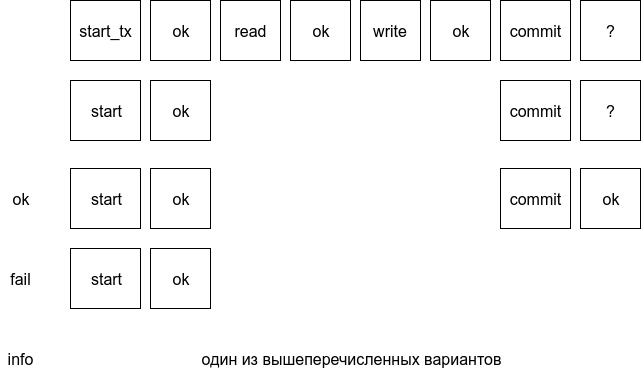
\includegraphics[scale=0.5]{history-transform.png}
    \caption{Преобразование истории. Каждая транзакция  в зависимости от
        статуса завершения может быть несколькими вариантами преобразована в две операции --
        чтения и записи соответственно.}
\end{figure}

\begin{itemize}
    \item Если $commit$ операция завершилась \textbf{fail}-записью, обе записи
        соответствующие $commit$ операции удаляются.
        $start$ операция преобразуется в $read$ операцию для того-же множества регистров.
        То есть не меняющее состояние объекта чтение.
    \item Если $commit$ операция завершилась \textbf{ok}-записью, то
        $start$-операция преобразуется в $read$ операцию, блокирующую регистры,
        в которые пишет $commit$ операция. Соответственно операция определена только на объектах,
        в которых соответствующие регистры не заблокированы. $commit$ операция преобразуется в
        $write$ операцию, при этом разблокирующую регистры в которые пишет.
        Соответственно определена только на объектах, в которых соответствующие регистры заблокированы.
    \item Если $commit$ операция не завершилась или завершилась \textbf{info}-записью, то рассматриваем два варианта истории,
        преобразованной одним из вышеупомянутых способов.
\end{itemize}

Таким образом получаем некоторое множество историй.
\begin{lemma}
    Snapshot-сериализуемость исходной истории равносильна линеаризуемости одной из историй, полученных
    приведённым преобразованием.
\end{lemma}
\begin{proof}
    В одну из сторон приведённое утверждение очевидно. То есть из snapshot-сериализуемости очевидна линеаризуемость
    одной из полученных историй. Пусть $T$ получена из $H$ и $L$ -- линеаризация $T.$ Покажем как построить линеаризацию
    $H$ удовлетворяющую \ref{snapshot-def}. Рассмотрим $L'$ соответствующую $L.$ В том смысле, что операции в $L'$ получаются
    из операций в $L$ игнорированием блокировки регистров. $read$-записям соответствуют $start$-записи,
    $write$ переходят в $commit$. Рассмотрим ограничение $L$ на один из регистров. Также удалим неблокирующие чтения.
    Из линеаризуемости $T$ очевидно, что чтения и записи чередуются, и история начинается с чтения.
    Покажем, что история устроена следующим образом: каждой записи предшествует соответствующее чтение(с тем же идентификатором
    процесса), устанавливающее блокировку и за каждым чтением следует соответствующая запись. От противного: пусть пара $u$, $v$
    -- последовательные чтение и запись с разными идентификаторами процесса. Тогда в истории должно присутствовать соответствующее
    $v$ чтение $w$. Более того, оно должно быть расположено перед $u.$ Тогда после него должна быть запись с другим идентификатором
    процесса. Получаем противоречие с тем что пара $u, v$ первая. Пусть теперь пара $u$, $v$ в $L'$ -- соответствующие $start$ и
    $commit$ операции. Пусть между $u$ и $v$ есть $w$ которая пишет в один из регистров, в которые пишет $v.$ Тогда ограничивая $L$ на
    этот регистр получаем противоречие вышедоказанному.
\end{proof}

Алгоритм устроен следующим образом:
\begin{itemize}
    \item Сначала строится преобразование истории: при неоднозначности преобразования элементом истории является кортеж альтернатив.
        У $ret$-записей альтернатив нет. Для некоторых записей помечаем что при выполнении следующую операцию
        данного процесса надо игнорировать.
    \item Удаляются все \textbf{fail} и \textbf{info} записи. Для \textbf{fail}-записей необходимо удалить также \textbf{call}-запись.
    \item Производится поиск в пространстве состояний, схожий с описанным в разделе \ref{cypress-verify}.
\end{itemize}

Состоянием так же является $\langle state, history \rangle.$
При вычислении смежных состояний мы рассматриваем все альтернативы для каждой \textbf{call}-записи, и удаляем
из истории следующую операцию процесса(если помечено что надо её проигнорировать).
При поиске запоминаем пройденные состояния, в том смысле что запоминаем пару (множество удалённых операций, состояние).
В \cite{horn-faster} запоминали именно пару $\langle state, history \rangle,$ что создавало некоторое замедление из-за
необходимости сравнения историй, которые хранились в неизменяемом односвязном списке. Авторы предлагают кешировать результаты
сравнения списков для ускорения работы алгоритма. Мы же, поддерживая множество удалённых операций(bitset) добились сравнимой
производительности при меньшей сложности алгоритма.

Как и в алгоритме, описанном в \ref{cypress-verify}, при постановке экспериментов,
перед началом работы алгоритма явно строится граф состояний и переходов для модели,
мемоизируется именно множество удалённых операций, но в отличие от \cite{knossos}, мы
используем неизменяемые списки, что с одной стороны замедляет алгоритм, но с другой позволяет
эффективно распределить вычисления на несколько процессорных ядер и результирующее время работы
(на синтетических тестах) получается меньше.

\begin{center}
  \begin{tabular}{| c | c | c | c | c| }
      \hline
        Номер теста & Длина истории & knossos & наша реализация \\
        \hline
        1           & 20            & 0.2с     & 2с             \\
        \hline
        2           & 200           & 40с      & 10с              \\
        \hline
        3           & 800           & 1200с    & 100с              \\
        \hline
  \end{tabular}
\end{center}
Все тесты производились на 16-ядерном процессоре, с доступным объёмом памяти 60G.

\chapter{Проведённые эксперименты}
\section{Кипарис}
Было исследовано поведение системы при следующих условиях.
\begin{itemize}
    \item Использовалась модель атомарного регистра, со следующими доступными типами операций:
        \begin{itemize}
            \item \textbf{read} -- Чтение значения регистра, возможны исходы:
                \begin{itemize}
                    \item \textbf{ok} -- Удалось прочитать значение регистра.
                    \item \textbf{fail} -- Не удалось прочитать значение.
                \end{itemize}
            \item \textbf{write} -- Запись в регистр, возможны исходы:
                \begin{itemize}
                    \item \textbf{ok} -- Удалось записать значение.
                    \item \textbf{fail} --  Хранилище отклонило операцию.
                    \item \textbf{unknown} -- Возможно удалось записать значение
                        (хранилище не отклонило и не подтвердило операцию).
                \end{itemize}
        \end{itemize}
        Соответственно, все операции с хранилищем производились по одному и тому же ключу.
    \item Запросы осуществлялись в 8 потоков, чтение с последователей разрешено.
    \item Для обнаружения ошибок в сетевую конфигурацию вносились сбои следующего вида:
    \subitem Кластер разбивался на две примерно равные части, также было исследовано поведение при разбиении
            на две равные части с одним узлом “перемычкой”, который видит остальные.
    \subitem Также было исследовано поведение алгоритма при периодических обрывах сети между текущим лидером
            и остальными узлами.
\end{itemize}
В исходной постановке считалось что исход любой неудавшейся записи -- \textbf{fail}.
После ряда экспериментов, были обнаружены аномалии вида "чтение неподтверждённых записей".
После анализа исходного кода, было обнаружено, что запросы записи нельзя однозначно считать отклонёнными системой.
В скорректированной постановке, ошибок линеаризации на данный момент обнаружено не было.

Все эксперименты проводились с rpc\_timeout=3000 на всех узлах.

Тест 1 -- успешно верфицировано соблюдение гарантий. Каждые две секунды теряется связь с текущим лидером.
Запросы делаются с промежутками в 0.3 секунды в 5 потоков.
Время сбора истории -- 40 секунд, время верификации 1 минута.

\begin{figure}[H]
    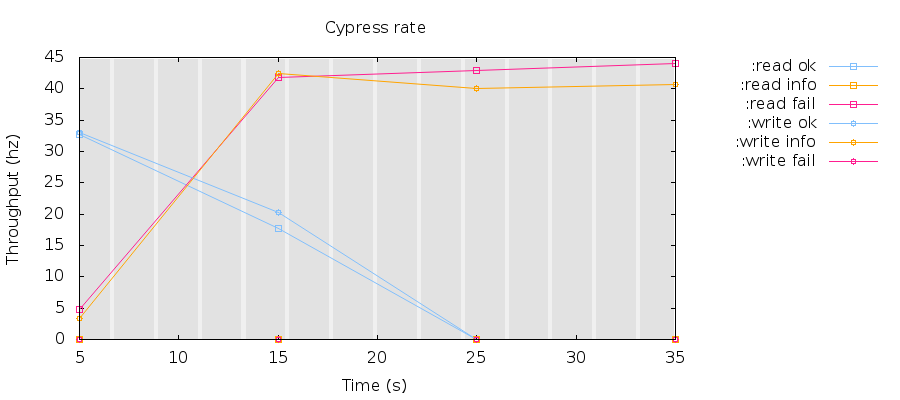
\includegraphics[scale=0.6]{cypress-2/rate.png}
    \caption{Частота запросов, тест 1}
\end{figure}

\begin{figure}[H]
    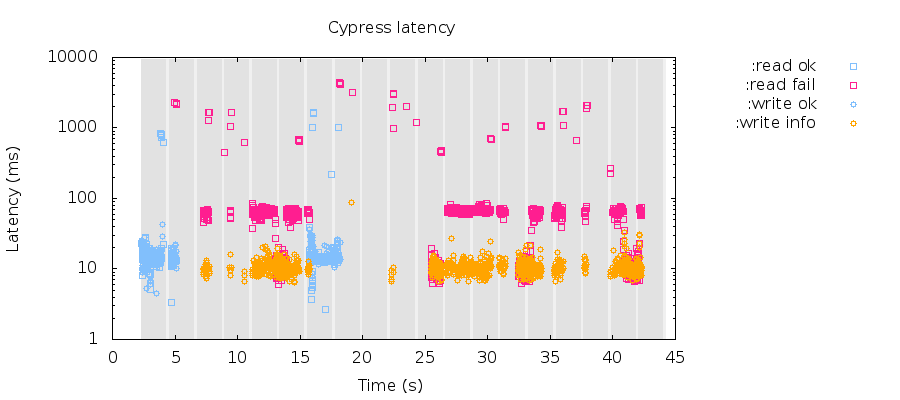
\includegraphics[scale=0.6]{cypress-2/latency-raw.png}
    \caption{Время отклика, тест 1}
\end{figure}

\begin{figure}[H]
    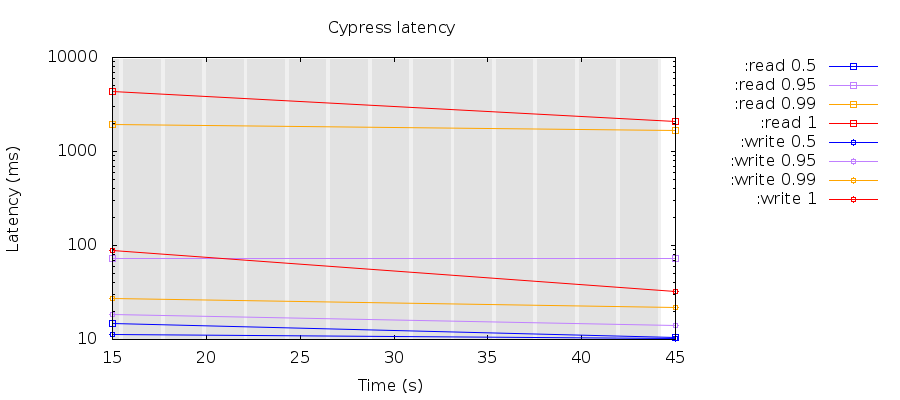
\includegraphics[scale=0.6]{cypress-2/latency-quantiles.png}
    \caption{Квантили времён отклика, тест 1}
\end{figure}

Тест 2 -- успешно верфицировано соблюдение гарантий. Каждые 6
секунд кластер делится на две примерно равные части.
Запросы делаются с промежутками в 0.3 секунды в 5 потоков.
Время сбора истории -- 40 секунд, время верификации 1 минута.

\begin{figure}[H]
    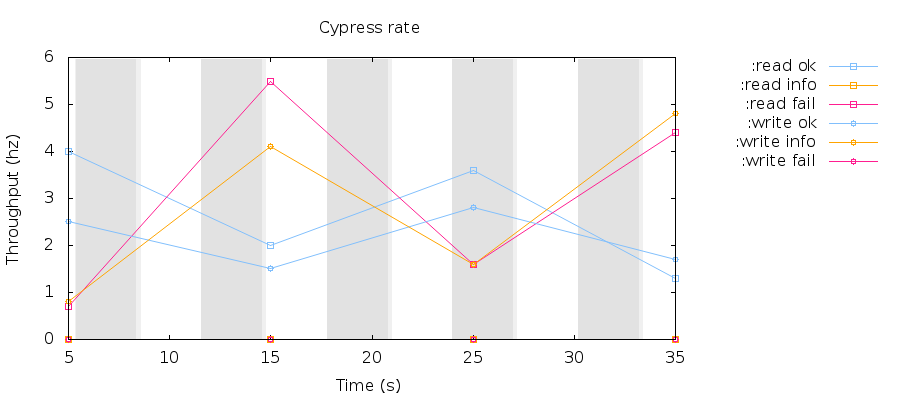
\includegraphics[scale=0.6]{cypress-5/rate.png}
    \caption{Частота запросов, тест 2}
\end{figure}

\begin{figure}[H]
    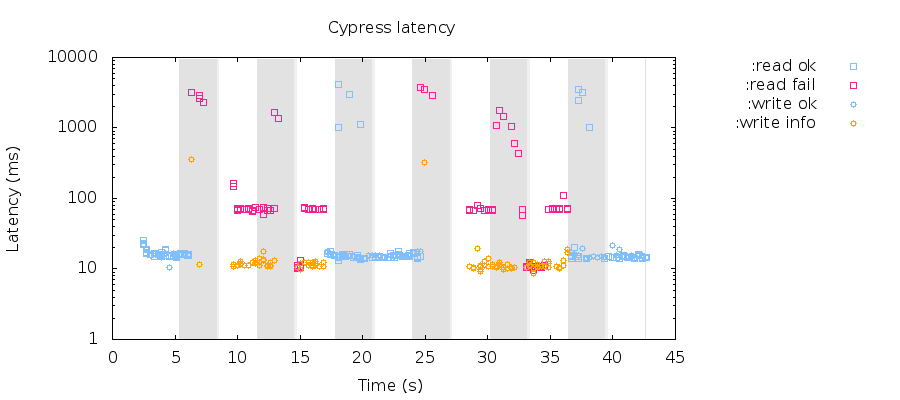
\includegraphics[scale=0.6]{cypress-5/latency-raw.png}
    \caption{Время отклика, тест 2}
\end{figure}

\begin{figure}[H]
    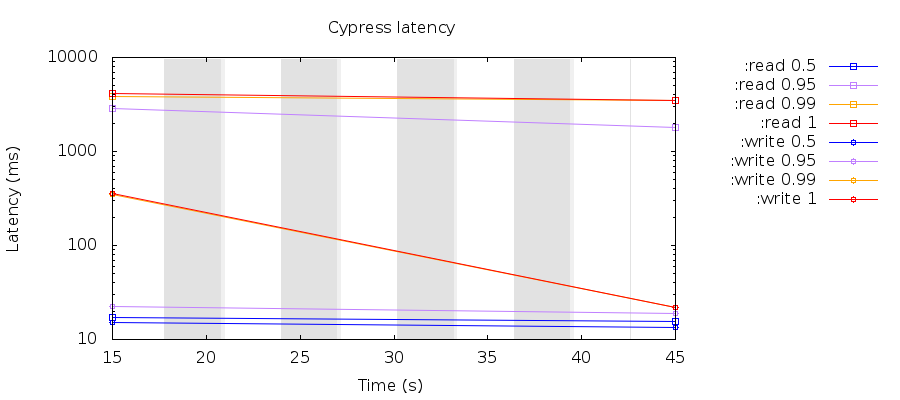
\includegraphics[scale=0.6]{cypress-5/latency-quantiles.png}
    \caption{Квантили времён отклика, тест 2}
\end{figure}

\section{Динамические таблицы}
Использовался алгоритм, описанный в \ref{dt-verify}.
Так как начало транзакции в исследуемой системе скорее логическое(клиент получает timestamp, и в дальнейшем
все чтения осуществляет по нему), то $start$ операции, завершившиеся по таймауту можно считать завершившимися
с \textbf{fail} статусом.
Было исследовано поведение системы при следующих условиях.
\begin{itemize}
    \item Размер кластера -- 5 узлов, 1 узел -- timestamp-provider, 5 шардов.
    \item Запросы осуществлялись в 6 потоков. Было исследовано поведение системы при записях
        на 1 шард и на 2 шарда(распределённые коммиты).
    \item Для обнаружения ошибок в сетевую конфигурацию вносились сбои следующего вида:
        \subitem Кластер разбивался на две примерно равные части.
        \subitem Избирательно обрывалась сеть между узлами, обслуживающими случайный шард и мастером.
\end{itemize}

В каждом шарде находится по одному ключу, по которому в дальнейшем и делаются запросы чтения/записи.

Все эксперименты проводились с rpc\_timeout=3000 на всех узлах.
Общий таймаут на транзакцию -- 6.3 секунд.

Тест 1 -- успешно верфицировано соблюдение гарантий. С перерывами по 8 секунд
обрывается связь с узлом обслуживающим один шард на 8 секунд. Каждая транзакция состоит
из двух чтений и двух записей. Запросы делаются с промежутками в 0.2 секунды в 5 потоков.
Время сбора истории -- 80 секунд, время верификации 11 минут.

\begin{figure}[h]
    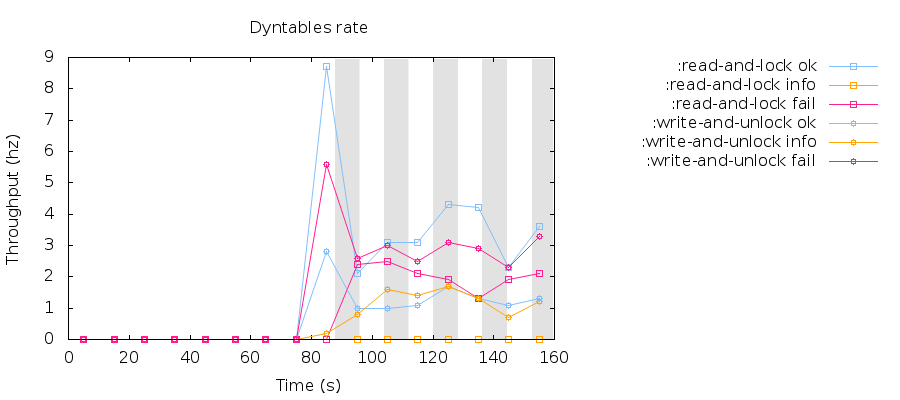
\includegraphics[scale=0.6]{dyntables-1/rate.png}
    \caption{Частота запросов, тест 1}
\end{figure}

\begin{figure}[h]
    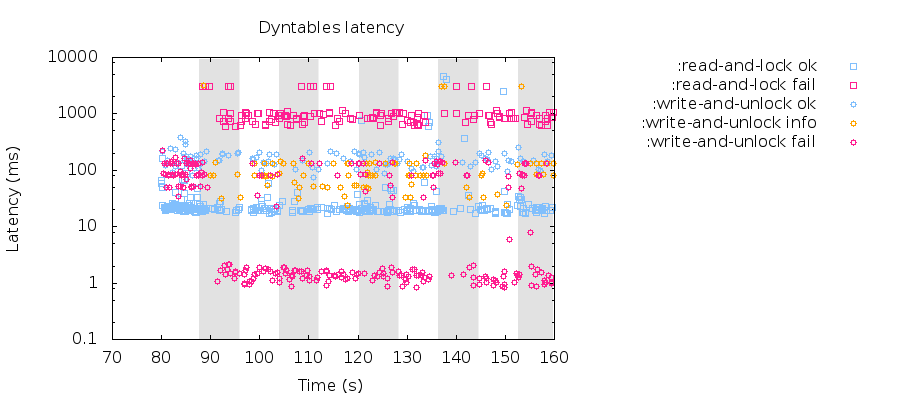
\includegraphics[scale=0.6]{dyntables-1/latency-raw.png}
    \caption{Время отклика, тест 1}
\end{figure}

\begin{figure}[h]
    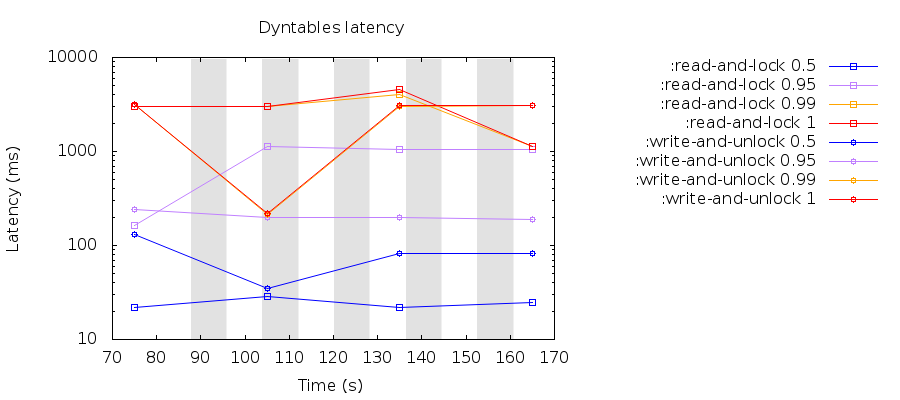
\includegraphics[scale=0.6]{dyntables-1/latency-quantiles.png}
    \caption{Квантили времён отклика, тест 1}
\end{figure}

Тест 2 -- успешно верфицировано соблюдение гарантий. С перерывами по 3 секунды
обрывается связь с узлом обслуживающим один шард на 8 секунд. Каждая транзакция состоит
из двух чтений и двух записей. Запросы делаются с промежутками в 0.2 секунды в 5 потоков.
Время сбора истории -- 80 секунд, время верификации 3 минуты.

\begin{figure}[h]
    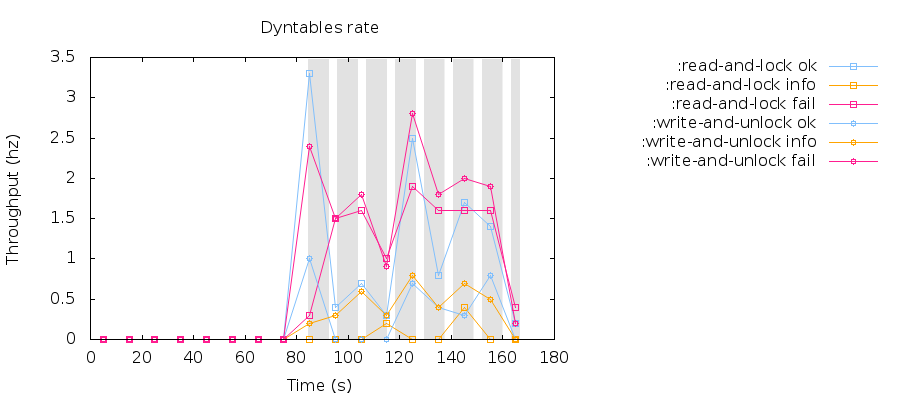
\includegraphics[scale=0.6]{dyntables-2/rate.png}
    \caption{Частота запросов, тест 2}
\end{figure}

\begin{figure}[h]
    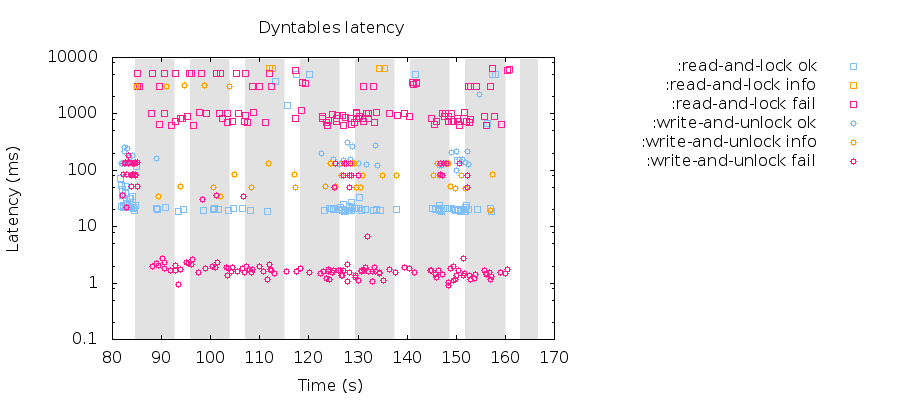
\includegraphics[scale=0.6]{dyntables-2/latency-raw.png}
    \caption{Время отклика, тест 2}
\end{figure}

\begin{figure}[h]
    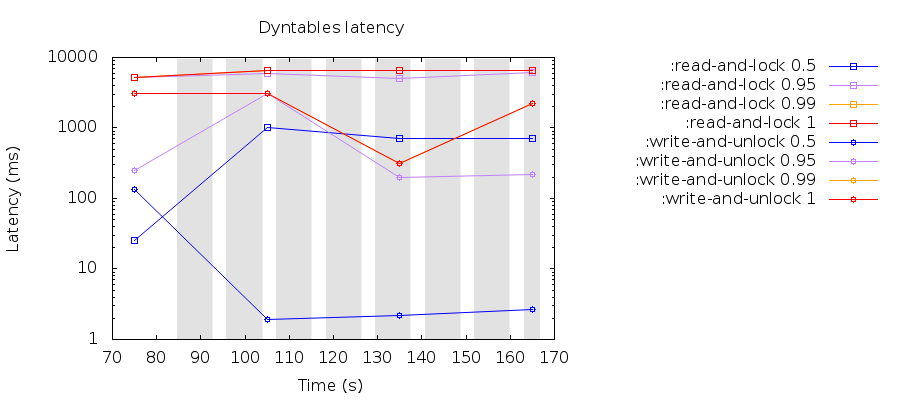
\includegraphics[scale=0.6]{dyntables-2/latency-quantiles.png}
    \caption{Квантили времён отклика, тест 2}
\end{figure}

Тест 3 -- успешно верфицировано соблюдение гарантий. С перерывами по 8 секунд
обрывается кластер делится на две примерно равные части, timestamp-provider доступен всем. Каждая транзакция состоит
из двух чтений и двух записей. Запросы делаются с промежутками в 0.2 секунды в 5 потоков.
Время сбора истории -- 80 секунд, время верификации 2.5 минуты.

\begin{figure}[h]
    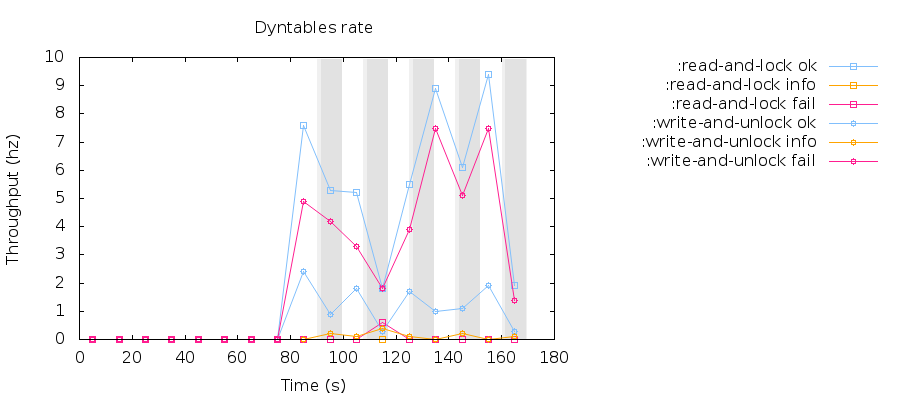
\includegraphics[scale=0.6]{dyntables-3/rate.png}
    \caption{Частота запросов, тест 3}
\end{figure}

\begin{figure}[h]
    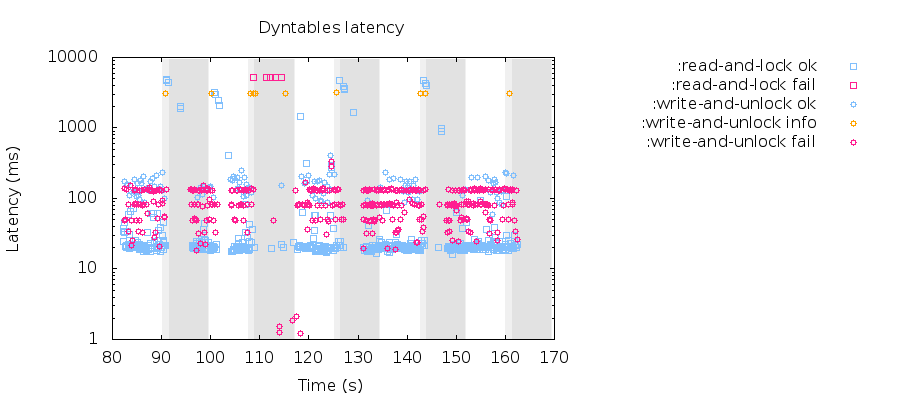
\includegraphics[scale=0.6]{dyntables-3/latency-raw.png}
    \caption{Время отклика, тест 3}
\end{figure}

\begin{figure}[h]
    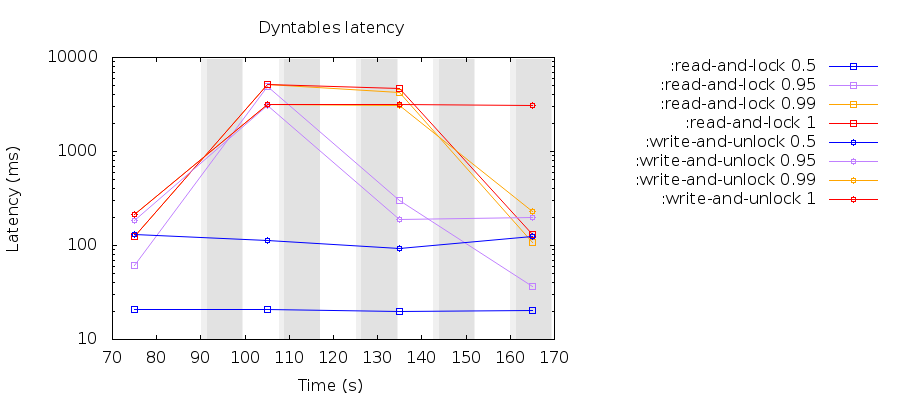
\includegraphics[scale=0.6]{dyntables-3/latency-quantiles.png}
    \caption{Квантили времён отклика, тест 3}
\end{figure}

Тест 4 -- успешно верфицировано соблюдение гарантий. С перерывами по 3 секунды
обрывается кластер делится на две примерно равные части, timestamp-provider доступен всем. Каждая транзакция состоит
из двух чтений и двух записей. Запросы делаются с промежутками в 0.2 секунды в 5 потоков.
Время сбора истории -- 80 секунд, время верификации 2.5 минуты.

\begin{figure}[h]
    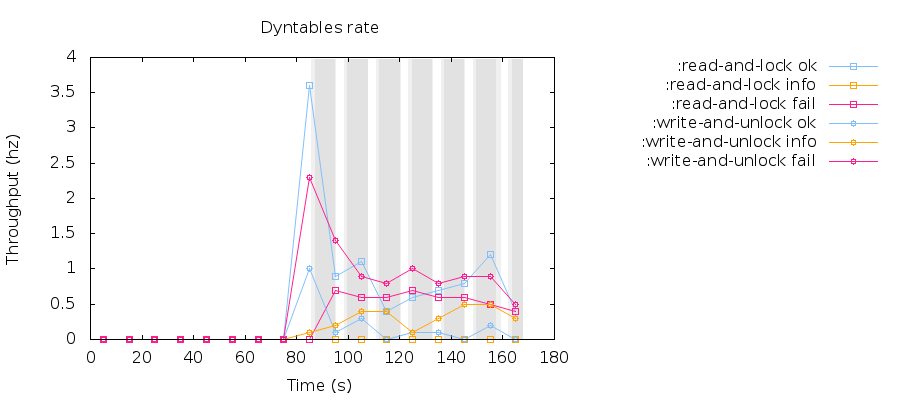
\includegraphics[scale=0.6]{dyntables-4/rate.png}
    \caption{Частота запросов, тест 4}
\end{figure}

\begin{figure}[h]
    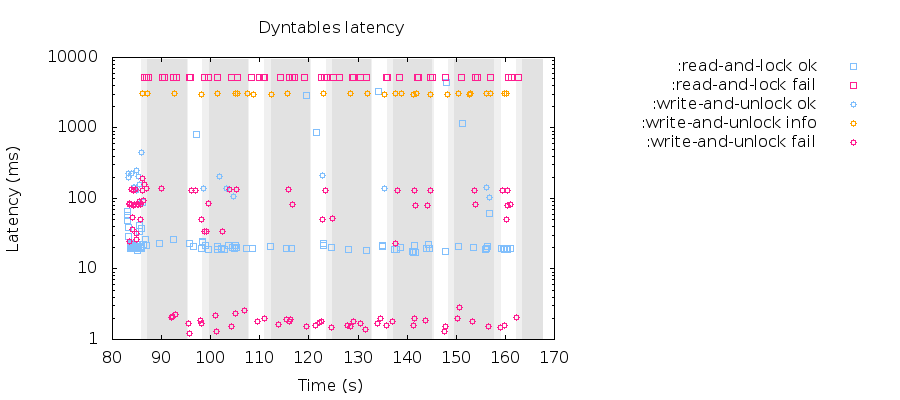
\includegraphics[scale=0.6]{dyntables-4/latency-raw.png}
    \caption{Время отклика, тест 4}
\end{figure}

\begin{figure}[h]
    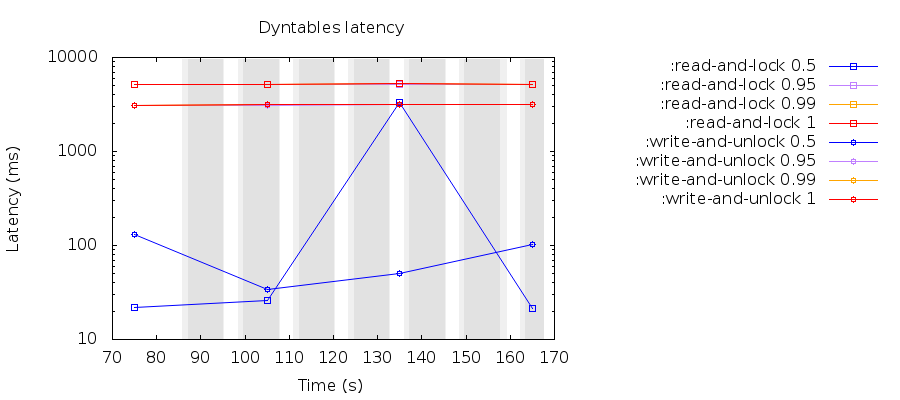
\includegraphics[scale=0.6]{dyntables-4/latency-quantiles.png}
    \caption{Квантили времён отклика, тест 4}
\end{figure}

Тест 5 -- Получена история не соблюдающая гарантии. С перерывами по 4 секунды
обрывается связь с двумя узлами обслуживающим какие-то шарды на 2 секунды. Каждая транзакция состоит
из двух чтений и двух записей. Запросы делаются с промежутками в 0.2 секунды в 5 потоков.
Время сбора истории -- 80 секунд, время верификации 1 минута, что неудивительно, так как в собранной
истории всего одна успешная операция.

\begin{figure}[h]
    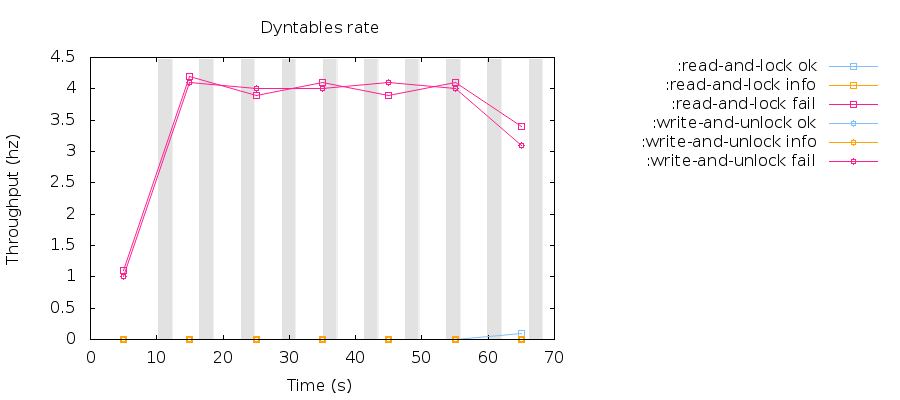
\includegraphics[scale=0.6]{dyntables-5/rate.png}
    \caption{Частота запросов, тест 5}
\end{figure}

\begin{figure}[h]
    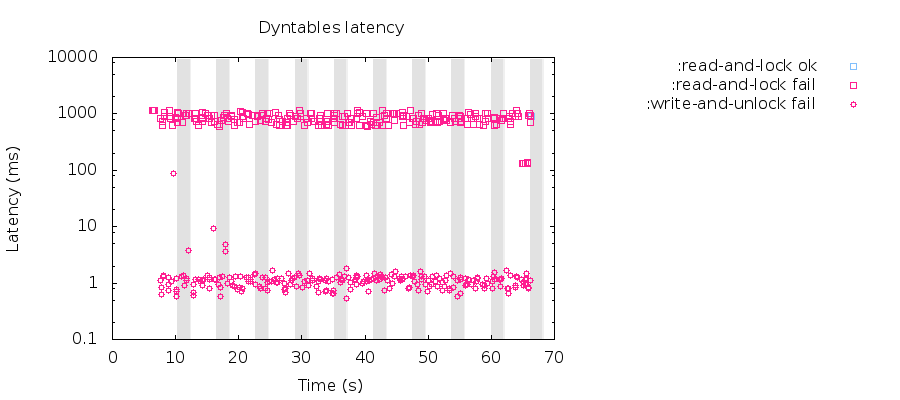
\includegraphics[scale=0.6]{dyntables-5/latency-raw.png}
    \caption{Время отклика, тест 5}
\end{figure}

\begin{figure}[h]
    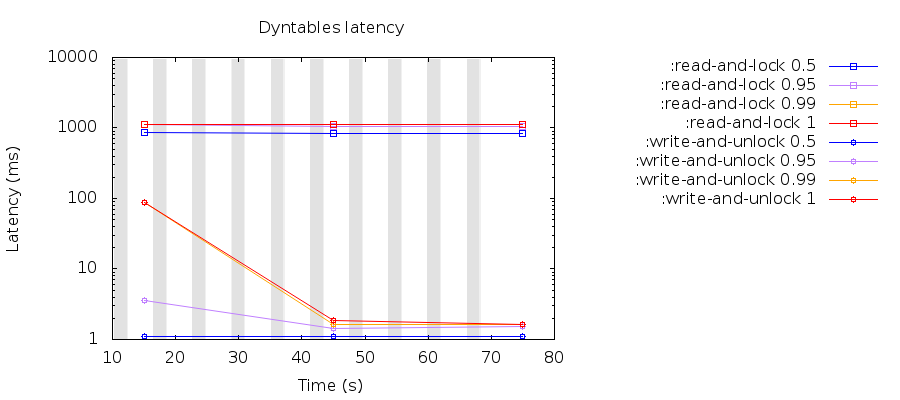
\includegraphics[scale=0.6]{dyntables-5/latency-quantiles.png}
    \caption{Квантили времён отклика, тест 5}
\end{figure}

\printbibliography[title=Список литературы]
\end{document}
